\chapter{文件系统部分设计与实现} 
% \pagenumbering{arabic} % 阿拉伯数字页码
\section{文件系统总体设计}
我们的简单内核目前肯定支持不了其他USB设备(除引导内核用的之外),不能进入系统后从USB设备拷贝文件,所以目前我们只能有两种方式可以
新建文件,一是从键盘输入,二是从内核而来.键盘输入显然有限,输入几MB字符不太现实,故需要从内核拷贝.这样才能
达到创建较大文件,测试文件系统的目的.这要保证静态内存分配的bss段要足够大.


我们要操纵的硬盘是哪一个呢?若是真实物理机测试的话,内核是存放于U盘的,我们的文件系统或许可以和内核
合成一块,做成系统集成盘,就像赵炯《Linux内核完全注释》中Linux0.11的实验环境一样.但是由于水平所限
,而且考虑到文件系统与内核分开实现起来可能更清晰一点,我采用分开的方法,文件系统和内核在不同的盘块上.

首先进行硬盘检测(init\_hd),如果说内核在IDE(ATA)硬盘0(hda),那么我们的文件系统需要建立在第二块IDE(ATA)硬盘2(hdb)上,所以若在物理机器上测试时,
应当确保第二块硬盘的存在.我们编写代码和平时调试时还是借助硬件模拟器qemu运行,
命令是这样qemu-system-x86\_64 -m 666 -hdb build/hd.img RiOS-i386.iso -monitor stdio
这条命令的意思就是内核镜像采用RiOS-i386.iso,它放在硬盘0即hda中;文件hd.img就作为硬盘1;虚拟机的内存设为666MB;对虚拟机
的监控信息重定向到字符设备.更多命令使用方法可通过qemu-system-x86\_64 -help查看,了解qemu使用之后亦可结合gdb调试.

建立文件系统,首先应当格式化全盘,因此如果要在实际的物理机器上测试,会有格式化全盘的危险,因此务必慎重.
一般还是在虚拟机qemu中运行,这个没有任何风险,大可放心.

磁盘读取硬盘分区表,判断特定位置有无magic number(这里是自己随意定的0x88),若无,则格式化全盘
建立文件系统;如果有,则说明是系统安装后第二次或更多次开机,不需要重新建立,只需要加载上次关机时的文件.

\section{物理硬盘}
\subsection{物理容量设定}

为方便代码和相关资料的传输,磁盘不宜过大,但也不能过小,否则体现不出文件系统的功能.
目前磁盘采用10MB,磁盘前一部分是一些控制信息,有引导扇区和inode位图和inode区等等.
考虑到这些也占空间,故设数据区8MB.我们的策略是:inode的管理采用位图法,空闲数据区磁盘
空间的管理采用成组链接的方法.

我们设数据区前8MB放除了专用块之外的空闲块,8* 1024 * 2=16384sectors,设数据区(专用块)
一共8*1024块,64块划分成一组,一共128块,专用块和普通的空闲块并没有什么本质上的不同.

在编写代码的时候,当然不必每次都在物理机器上测试,因此采用10MB大小的文件hd.img作为虚拟硬盘.

\subsection{磁盘格式化}

初始化时,若之前未初始化,先指定第一组的第一块为专用块,把此块复制到内存专用块中;如果已经初始化,
从磁盘加载超级块到内存,得到专用块的块号.所有组的第一块相互链接,初始化时类似一个顺序表,
这些组的第一块第一项存空闲块计数,第二项存下一块的块号,当专用块用完时,它就指定它的下一块是专用块,
并在超级块中更改专用块的块号.所有组的第一块相互链接,类似一个顺序表,这些组的第一块第一项存空闲块计数,
第二项存下一块的块号,当专用块用完时,它就指定它的下一块是专用块,并在超级块中更改专用块的块号.
组号写代码时从1开始编号.

磁盘初始化时即格式化磁盘,若采用在qemu虚拟机上测试的方法,则需要利用bochs的工具来制作一个10MB的空白磁盘镜像,
其方法是,在Linux终端输入bximage,然后依次选择输入hd, flat, 10, rios\_hd.img
就能得到一个名为rios\_hd.img的10MB大小磁盘镜像;若在真实的物理机器上测试,格式化磁盘将会在函数init\_hd中发生,
清空磁盘,此举有一定的危险性,如果想要进行下去,请务必确认您的电脑中没有重要资料,否则将被格式化.

\subsection{目录项的确定}

如何得知一个目录文件里有多少个目录项?目录文件的inode中记录有大小i\_size,由目录文件的inode
中的i\_size得到目录文件大小.而struct dir\_entry目录项的大小是固定的,由i\_size除以 sizeof(dir\_entry)
可知有几个目录项目.


\section{硬盘驱动}
IDE硬盘中的IDE不是集成开发环境的缩写,而是"Integrated Drive Electronics"的缩写,IDE硬盘又名ATA硬盘.
我们的内核处于IDE硬盘0上,首先检测hdb即IDE硬盘1是否存在(judge\_disk1\_exist),x86.h中通过outb(port,value)
和inb(port)两个宏定义简单包装了in、out指令,然后向硬盘发送相应指令,这里需要查阅IDE/ATA硬盘的手册,或者可以
到osdev网站上了解一下背景知识(https://wiki.osdev.org/ATA\_PIO\_Mode).
ATA硬盘通过0x1F0至0x1F7这8个端口再加一个0x3f6端口来控制.以下表格(图~\ref{ATA_ports}~)定义了0x1F0至0x1F7这8个端口的功能,

\begin{figure}[!htbp]
	\centering	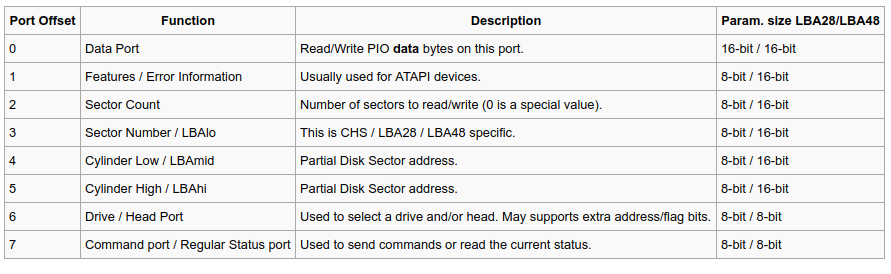
\includegraphics[width=14cm]{pic/assets/ATA_ports}
    \caption{ATA硬盘0x1F0至0x1F7端口的功能}	\label{ATA_ports}	\end{figure}
% \begin{tabular}{|c|c|c|c|}% 通过添加 | 来表示是否需要绘制竖线
%     \toprule
% 	Port Offset& 	Function	& Description	& Param. size LBA28/LBA48\tabularnewline
%     \midrule
% 	0	& Data Port	& Read/Write PIO data bytes on this port.& 	16-bit / 16-bit\tabularnewline
% 	1	& Features / Error Information & 	Usually used for ATAPI devices.& 	8-bit / 16-bit\tabularnewline
% 	2	& Sector Count	& Number of sectors to read/write (0 is a special value).	& 8-bit / 16-bit\tabularnewline
% 	3	& Sector Number / LBAlo	& This is CHS / LBA28 / LBA48 specific.	8-bit / 16-bit\tabularnewline
% 	4	& Cylinder Low / LBAmid & 	Partial Disk Sector address.	& 8-bit / 16-bit\tabularnewline
% 	5	& Cylinder High / LBAhi & 	Partial Disk Sector address.	& 8-bit / 16-bit\tabularnewline
% 	6	& Drive / Head Port	& Used to select a drive and/or head. May supports extra address/flag bits.	& 8-bit / 8-bit\tabularnewline
% 	7	& Command port / Regular Status port & 	Used to send commands or read the current status.	& 8-bit / 8-bit\tabularnewline
%     \bottomrule
% \end{tabular}

硬盘有三种访问模式,一是"CHS mode",即通过柱面(Cylinder)、磁头(Head)、扇区(Sector)来访问,这种方式
相对比较麻烦,而且能访问到的容量有限;二是"LBA28 mode";三是"LBA48 mode".前两种方法已经过时了,用"LBA48 mode"
可以访问更大的容量,而且更为方便,我们采用的是"LBA48 mode".

通过get\_hd\_size(0)和get\_hd\_size(1),我们分别得到了hd1和hd2的硬盘容量.因为我们的文件系统建立在硬盘1(hdb)上,
通过端口,发送命令切换到hdb(switch\_to\_disk(1)).

\subsection{选择IDE(ATA)硬盘}



\subsection{硬盘读写}
这里仅是写,读也类似,使用的是LBA访问方式,由于一次传不了很长的地址,需要把地址拆开成几段,
依次传输,这里需要查阅ATA硬盘的相关资料(推荐到osdev.org查阅).用这种访问磁盘的方式,写出来
都大同小异,只需要符合规范即可.这里确保是针对硬盘1进行读写,存放内核的硬盘0不去动它.

\begin{minted}{c}
void IDE_write_sector(void *src,int lba)
{
	switch_to_disk(1);
	set_disk_no(1);/*disk1 :PC hard disk */
	IDE_disk_wait();
	outb_wait(ATA_PORT_SECT_COUNT,1);/*outb(0x1f2,1);*/
	outb_wait(ATA_PORT_LBA_LOW ,lba);/*outb(0x1f3,lba);*/
	outb_wait(ATA_PORT_LBA_MID ,lba >> 8);/*outb(0x1f4,lba>>8)*/
	outb_wait(ATA_PORT_LBA_HIGH ,lba >> 16);/*outb(0x1f5,lba>>16)*/
	outb_wait(ATA_PORT_DEVICE , 0xe0 |(disk_no&1)<<4| (lba >> 24));/*outb(0x1f5,lba>>16)*/
	/*disk_no determines write to which disk.*/
	outb_wait(ATA_PORT_STATUS, HD_WRITE);
	IDE_disk_wait();
	for(int i = 0; i < SECTOR_SIZE/4 ; i++){
	     _out_data32(ATA_PORT_DATA,((u32*)src)[i]);
	}
}
\end{minted}
\section{建立硬盘分区表}
这里有关于硬盘分区表的简单介绍(http://www.gotothings.com/unix/disk-partition-table.htm).


\section{基于位示图的inode分配与回收}
位示图的方法比较简单.在
\begin{minted}{c}
	int new_inode()
	{
		u8 sector[512]={0};
		int i = 0;rios_superblock.s_startsect = 1;
		IDE_read_sector((void *)&sector,NR_INODE_MAP_BLK(rios_superblock));
		for(i=0;i<512*8;i++){
			if(bitmap_test_bit(i,sector)){
				;
			}else{
				bitmap_set_bit(i,sector);
				IDE_write_sector((void *)&sector,NR_INODE_MAP_BLK(rios_superblock));
				return i;
			}
		}
		return i;
	}
\end{minted}	
\section{建立根目录}
这里要申请inode号并分配数据区,建立"."和"..",如果是初次建立文件系统,
应当把系统中默认的目录如/usr等建立好,创建大文件jane.txt和小文件hamlet.txt
留待测试用.第二次"make run"或"make qemu"进系统时就不需要做这些了.

\section{基于成组链接法的磁盘空闲块管理}
\begin{minted}{c}    
int new_block()
{
	union Super_Block_Sect *p_ri_sb = get_super();
	set_super();
	if(!is_specific_block_set){
/*initially, the first( counting from 1 ) data block is allocated for specific block.*/		
		p_ri_sb->s_specific_blk_nr = 1;set_super();/*write back to disk*/
		specific_block = get_blk_nr_free_group(p_ri_sb->s_specific_blk_nr);
		is_specific_block_set = 1;
	}
/* remember to write back to disk. */	
again:	
	if(specific_block.s_free > 1){
		specific_block.s_free --;
		set_specific_blk_nr(p_ri_sb->s_specific_blk_nr);/*write back*/
		set_blk_nr_free_group(specific_block,p_ri_sb->s_specific_blk_nr);
		return specific_block.s_free_blk_nr[specific_block.s_free];
	}else if(specific_block.s_free == 1){
		specific_block.s_free --;
		int current_group_nr = p_ri_sb->s_specific_blk_nr;
		int next_group_nr = specific_block.s_free_blk_nr[0];
/* get NR of next group,copy its contents to specific block in memory through buffer
 * , and **allocate current block**. 
 */
		specific_block = get_blk_nr_free_group(next_group_nr);
		set_specific_blk_nr(next_group_nr);
/* now, we are switching to a different specific block*/		
		specific_block.s_free --;
/* XX return specific_block.s_free_blk_nr[specific_block.s_free];
 * ok,we were able to return NR here,but in that case,the following code won't execute,
 * and the last specific block haven't been allocated.
 */		
		int tmp = specific_block.s_free_blk_nr[specific_block.s_free];
		{/* allocate the last specific block */
			specific_block.s_free_blk_nr[specific_block.s_free] = current_group_nr; 
			specific_block.s_free ++; 
		}
		if(tmp!=0){
/*write back*/
			set_blk_nr_free_group(specific_block,p_ri_sb->s_specific_blk_nr);
			return tmp;
		}else{/*SHOULD NOT allocate root*/
			goto again;
		}
	}else if(specific_block.s_free == 0){
		_panic(" FBI WARNING:There is no free block available!!!");
	}	
}
\end{minted}
\section{超级块设计}
超级块的s\_magic为rifs文件系统的魔幻数字,这里我设其为0x88,开机时若在磁盘上
超级块对应位置探测到0x88,系统就认为已经安装rifs文件系统.以下为磁盘超级块结构.

\subsection{硬盘超级块}
\begin{minted}{c}    
struct d_super_block
{
u16 s_ninodes;
u16 s_capacity_blks;/*capacity count in blocks*/
u16 s_startsect;/*超级块的起始扇区,sector0为boot sector,故超级块从1开始*/
u16 s_zone_bitmap_blks;/*according to Prof Jiang,we will not use this policy (data block bitmap) anymore.*/
u16 s_inode_bitmap_blks;/*num of blks that bitmap takes up*/
u16 s_inode_blks;
u16 s_firstdatazone;
u16 s_specific_blk_nr_group;/*成组链接专用块对应磁盘上的组号*/
u16 s_magic;/*ri_fs magic:0x88*/
};    
\end{minted}

\section{inode设计}
\subsection{内存中inode结构(m\_inode)}
\begin{minted}{c}   
struct m_inode
{
	u8 i_mode;			/*file type(dir/normal) and attribute(rwx)*/
	u8 i_uid;			/*user id*/
	u8 i_gid;			/*group id*/
	u8 i_nlinks;			/*num of files that link to it*/
	u8 padding0[2];
	u32 i_creat_time;	
	u16 i_zone[10];
	u16 i_ino;			/*inode id号 (bitmap)*/
	u32 i_size;			/*size of file*/
	u32 padding1[7];		/*占位 8*32个字节*/
/* ok,let's make sizeof(d_inode) exactly equal to 64,that's 512bits,
 * a sector can put exactly 8 of d_inode.
 * if we attemp to extend the m_inode and d_inode,make sure that
 * they are in sync with each other,and adjust the fields and paddings
 * without changing the sizeof(d_inode)
 * zone[0~6]:	direct block 
 * zone[7]:	single indirect block
 * zone[8]:	double indirect block 
 * zone[9]:	trible indirect block
 *These are only in memeory*/
	u32 i_access_time;
	u8 i_mount;
	u8 i_dev;			/*hd0 or hd1*/
	u8 i_dirty;
	u8 i_updated;
	u8 i_count;			/*引用数*/
	struct task_struct *i_wait;	/*not implemented yet*/
}__attribute__((packed));		/*一定要加,不然字节对不齐,会多用空间*/
\end{minted}

请控制好d\_inode的大小以及与m\_inode同步性.这里设置几个padding的意义在于占位,
我把d\_inode 的大小控制在8*6+32+16*10+16+32*8=512 bits,这样一个扇区512*8=4096bits,
正好可以放8个d\_inode,尽量避免跨扇区操作inode.

磁盘inode和内存inode的数据结构上相似,即内容上磁盘inode结构是内存inode结构的子集,
内存inode不但要保存磁盘inode的所有信息,还要保存进程和系统运行中的相关信息.为避免操纵磁盘inode时跨扇区操作,
这里我严格控制d\_inode结构体的大小,为512bits,即64B,而一个扇区512B,恰好可以放8个磁盘inode,
这里attribute((packed))很重要,如果不加的话,编译器为了字节对齐,一个结构体将使用多于64B的空间,
这样将导致inode的存放很碎,操作出问题.机构体里的padding主要是为了占位,凑到恰好64B,日后若扩展d\_inode时,
就减少padding的数量,然后加上要增加的新项,保持sizeof(struct d\_inode)不变.

\subsection{iget和iput}
内存中有inode的拷贝,iget和iput功能就是从硬盘上拷贝inode到指定内存或把内存中inode拷到硬盘.
有时会出现"脏数据"的情况,所以要特别注意内存与硬盘上信息的同步,不要忘记写回.

\section{目录管理}

\subsection{列出目录(ls)}
显示当前路径下有什么.

\subsection{创建和删除目录(mkdir、rmdir)}

有了在当前目录创建一级目录的基本操作以后,名字的分割是创建多级目录的关键,
比如要递归创建"dir1/dir2/dir3",要如何依次分解出dir1、dir2、dir3呢?
C标准库中解决这个问题对应着一个函数strtok,在string.h中.strtok该函数返回
被分解的最后一个子字符串,如果没有可检索的字符串,则返回一个空指针。string.h
中strtok的实现并不长,然而十分高效,也具有鲁棒性.要我写出这个函数是不出来的
,我们也不需要彻底重复制造轮子,那就借用一下库函数string.h的实现吧.这里函数
\mintinline{c}!char * strtok(char * s,const char * ct)!一共18行代码,
源于Linux2.4/lib/string.c,特此说明.

\begin{minted}{c} 
char *strtok(char s[], const char *delim);
//库函数strtok用法:分解字符串为一组字符串。s为要分解的字符串,delim为分隔符字符串。
\end{minted}

根据里奇的"KISS"懒汉原则,我把目录管理和文件管理的函数做到尽量傻瓜,比如mkdir函数只
支持在当前目录创建目录,至于多级目录的创建,则通过其他函数分解字符串,拆出各个单级目录
名,分别调用mkdir函数来实现mkdir dir1/dir2/dir3这样的功能,其他诸如cd dir1/dir2/dir3
也类似,不再重复说明.

在本系统中,不允许在同一目录创建同名文件夹.创建目录首先给目录分配inode和数据区,由于一个目录项所占空间是一定的,
故可以通过一个目录的大小除以目录项的大小得到目录的总数.

目录名长度有效,超过长度就报错.创建一个新目录时,应当先首先给它添加两个目录项指向自身的"."和父目录"..",
然后更新目录的大小.写回到磁盘.

删除目录也类似,要归还数据区和inode号.不过当要删除的目录不为空的情况下,不允许删除目录的操作.

\subsection{hexdump}
在DOS下学习汇编时会有以十六进制查看一块数据区的情况,Linux中也有类似的hexdump命令.
为了方便调试,更方便地找出问题,本系统也提供简单的hexdump命令,只提供最基本的功能.

图~\ref{hexdump523}~展示了硬盘1的第523扇区的内容.
\begin{figure}[!htbp]
    \centering	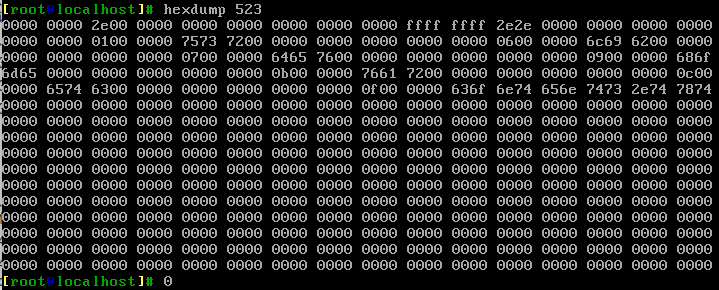
\includegraphics[width=14cm]{pic/assets/hexdump523}
	\caption{hexdump523}	\label{hexdump523}	\end{figure}
	
可以看到出现了十六进制的2e,不远处还有连续的两个2e,通过man ascii命令查ASCII码表可知这是"."和
"..".因此这是一个目录的数据区.

图~\ref{wxHexEditor}~是用wxHexEditor软件查看rios/build/hd.img的磁盘镜像.
\begin{figure}[!htbp]
    \centering	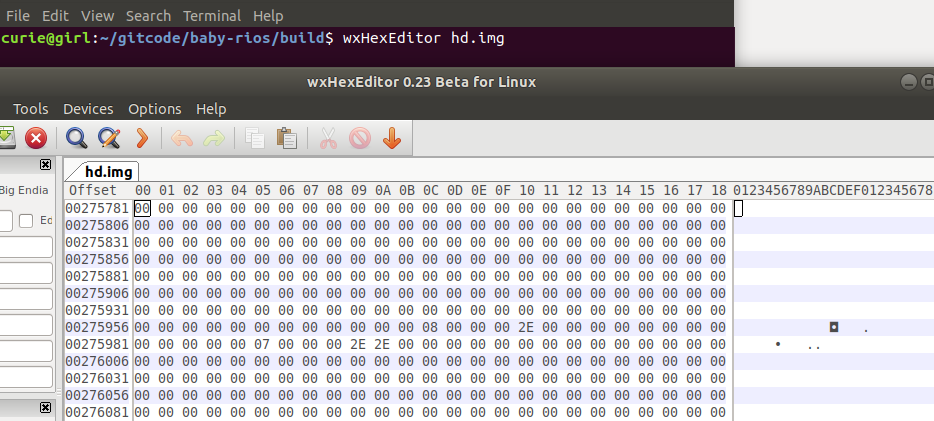
\includegraphics[width=14cm]{pic/assets/wxHexEditor}
	\caption{wxHexEditor}	\label{wxHexEditor}	\end{figure}
	
利用虚拟机编写测试时,我们也可以通过sublime软件打开rios/build/hd.img文件,这样直接
观测到"硬盘"上的数,可以与我们在系统中"hexdump 扇区号"得到的结果相比对,以验证hexdump的正确性. 
	
\subsection{切换目录(cd)}
支持多级切换,如cd dir1/dir2/dir3.多级的原理也是分解路径,和mkdir类似.

\paragraph{查看当前目录(pwd)}

使用pwd命令


\section{文件管理}
这里有三个关键的表,有:主存活动inode表、系统打开文件表、用户打开文件表.
他们的结构如下.

1.活动inode表.
\begin{minted}{c}
	struct active_inode_table{
		struct m_inode inode_table[MAX_ACTIVE_INODE];
	};   
\end{minted}

2.系统打开文件表:

\begin{minted}{c}
struct file file_table[NR_FILE];	   
\end{minted}

文件表整个系统中只有1张。该表可以视为结构体数组.

3.用户打开文件表(下面其中一个数据项):

进程控制块task\_struct
\begin{minted}{c}
	struct task_struct{
		u8 gid;
		u8 uid;
		struct m_inode * pwd;
		struct m_inode * root;
		struct file * filp[NR_OPEN];	/* 进程表项 */
	/* this is user-wide file table */	
	};	   
\end{minted}

理论上应该包含于进程PCB之中,每个进程有一份.

进程PCB记录当前的组id和用户id,内存inode指针pwd指向当前目录的inode,
内存inode指针指向当前根目录的inode,进程表项\mintinline{c}!struct file * filp[NR_OPEN]!,
为用户打开文件表.

由于工作量的问题,我没有做进程管理,但是为了可扩展性,还是定义了task\_struct,
用户打开文件表是进程表项,对应task\_struct里的\mintinline{c}!struct file * filp[NR_OPEN]!
.文件描述符表,每个进程有且仅有1张。该表可以视为指针数组,数组的元素指向文件表的一个元素。
最重要的是:数组元素的下标就是文件描述符。

这三个表中,活动inode表从磁盘上拷贝inode,另外由于表中结构体是struct m\_inode,
还存一些系统运行时的相关信息,比如内存m\_inode中的i\_count即被引用次数.
系统打开文件表file\_table其表中项的结构是file,file中包含指向m\_inode的指针,
即指向活动inode表的表项.用户打开文件表filp[NR\_OPEN],其中表项的结构是* file,即文件的指针.
文件描述符fd是filp[..]指针数组的index下标,fd可以看做file索引的索引.



\subsection{文件的打开和关闭}

\paragraph{文件结构} file:

\begin{minted}{c}
	struct file
	{
		u8 f_mode;			        /*文件读写模式及权限管理*/
		u8 f_flags;
		u16 f_count;			    /*file引用次数*/
		struct m_inode * f_inode;	/*指向活动inode表中文件的inode*/
		u32 f_pos;
	};	
\end{minted}

\paragraph{目录项结构} dir\_entry

\begin{minted}{c}
struct dir_entry{
	u32 inode;
	u8 name[MAX_NAME_LEN];
}__attribute__((packed));
\end{minted}


这里目录项对应目录中的一条记录的结构,记录两项内容,一是inode号,二是文件或目录名字.

\subsection{open}
open函数的功能是:给它输入文件名,然后返回有效的文件描述符.
首先按名查找,在当前目录根据文件名找到要打开的文件的inode号,
新建一个i节点表元素,让其对应打开的物理文件(如果对应于该物理
文件的i节点元素已经建立,就不做任何操作);

让其指向刚建立的文件表元素。最后将该元素的下标作为open的返回值返回。

这样当调用read(write)时,根据传入的文件描述符,操作系统就可以找到对应
的文件描述符表元素,进而找到文件表的元素,进而找到i节点表元素,从而完成对物理文件
的读写。




\begin{minted}{c}   
int open(const char *name){
	int fd,i;
	int ino = get_dir((char *)name);
	if(ino==0){
		kprintf(" open:failed, ino cannot be zero.");
		return -1;
	}
	if(ino==-1){
		kprintf("\n open: '%s':no such file or directory.",name);
		return -1;
	}
/* search the active inode table, if it's not in this table,just copy.*/	
	for(i=0;i<MAX_ACTIVE_INODE;i++){
		if(active_inode_table.inode_table[i].i_ino == ino)
			break;
	}
	int active_inode_table_nr=get_active_inode_table_nr();
	if(i>=MAX_ACTIVE_INODE){/*no record found,need to copy. */
		if(active_inode_table_nr>MAX_ACTIVE_INODE)_panic("FBI_WARNING:CAN NOT open more than 64 files at the same time!");
		iget(&active_inode_table.inode_table[active_inode_table_nr],ino);

	}else{/* it has been opened before, no nead to copy */
	      /* here,we get i */
		if(current->filp[i]->f_inode->i_ino == ino)return i;
		goto comeon;
	}
comeon:	
/* find a blank entry in process's file descriptor table */	
	for(fd=0 ; fd <NR_OPEN ; fd++ ){

		if(!current->filp[fd])
			break;
	}
	if(fd>=NR_OPEN)
		return -1;/* overflow */
/* find a blank entry in system file table */	
	file * p_ft = file_table;
	int j;
	for(j=0;j<NR_FILE;j++,p_ft++){
		if(!p_ft->f_count) break;
	}
	if(j>=NR_FILE){
		kprintf("\n failed to create.");
		return -1;
	}
	int valid_file_table_nr = j;
/* ok, let filp[fd] points to a entry in file table,and let f_count+=1 */
(current->filp[fd]=p_ft)->f_count++;
/* NOTICE! here we should let filp[fd]->f_inode point to an entry in active_inode_table*/
current->filp[fd]->f_inode = &active_inode_table.inode_table[active_inode_table_nr];
/* keep there tables in sync with each other */
	return fd;
}
\end{minted}

\subsection{多级索引}

系统中jane.txt这个文本文件有几MB大小,装下了《Jane Eyre》这部英文小说的全部内容,
大小足够测试了.

用cat jane.txt可以成功显示全书内容.如图~\ref{cat_jane}~所示

\begin{figure}[!htbp]
	\centering	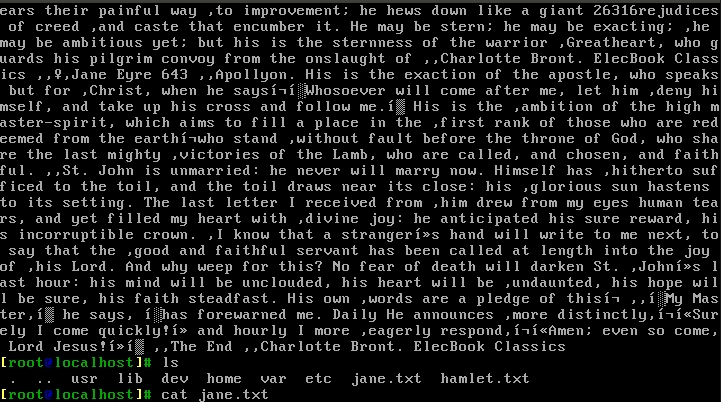
\includegraphics[width=14cm]{pic/assets/cat_jane}
	\caption{用cat命令查看jane.txt文本文件内容}	\label{cat_jane}	\end{figure}

cat显示命令比较快,一分钟之内可以把整本书的内容输出.用slowcat jane.txt也可以显示全书内容,
但速度很慢.如图~\ref{cat_jane}~所示.	

\begin{figure}[!htbp]
		\centering	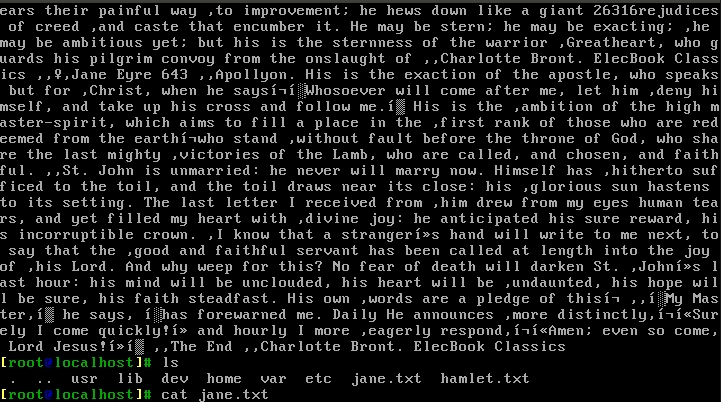
\includegraphics[width=14cm]{pic/assets/cat_jane}
		\caption{用slowcat命令查看jane.txt文本文件内容}	\label{cat_jane}	\end{figure}

\subsection{读写文件与删除文件}

由于是多级索引,删除文件实现起来比较麻烦,这里留到关键函数实现中谈.

\subsection{查看文件内容(cat)}

如图~\ref{cat_hamlet}~所示

\begin{figure}[!htbp]
	\centering	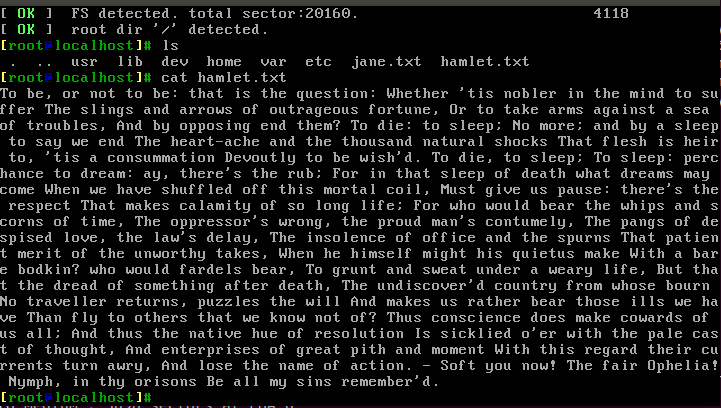
\includegraphics[width=14cm]{pic/assets/cat_hamlet}
    \caption{用cat命令查看文本文件内容}	\label{cat_hamlet}	\end{figure}

\subsection{查看硬盘1结构组成}
用自定义命令info disk查看,硬盘1由引导扇区(我们的内核在硬盘0,这里作用不大)、超级块、
废弃的数据区位示图区、inode区和数据区组成.本来准备使用位示图完成数据区的空闲空间管理
,后来应老师要求,改为成组链接方式,因而数据区的位示图区废弃不用.关于系统中命令的用法,
可通过help命令查看.

硬盘1结构组成如图~\ref{disk}~所示.

\begin{figure}[!htbp]
	\centering	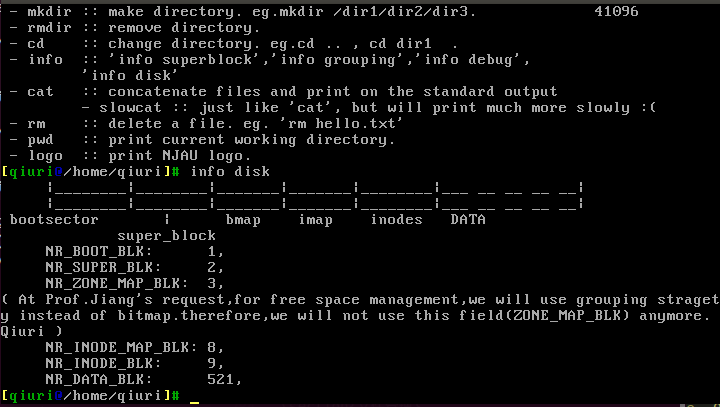
\includegraphics[width=14cm]{pic/assets/disk}
    \caption{硬盘1结构组成}	\label{disk}	\end{figure}








% \clearpage
